\section{Princípio da demanda efetiva no médio prazo e a estabilidade fundamental}
\label{Medium}

Da discussão anterior, verifica-se que a literatura sobre investimento residencial é bastante escassa nos modelos com gastos autônomos. Como será apresentado no capítulo seguinte, parte da literatura empírica (diminuta, mas crescente) destaca a importância deste componente da demanda para a dinâmica da economia norte americana. Diferentemente de grande parte dos trabalhos teóricos e empíricos, argumenta-se que é o investimento residencial que antecipa o ciclo econômico. Tal discussão é endereçada no capítulo seguinte, mas antes resta especificar qual modelo o mais adequado para o capítulo \ref{CapModelo} e isso é feito a seguir.



Para encerrar essa discussão, é feita uma comparação entre as duas alternativas restantes, qual sejam, Kalekiana não-convencional e Sraffiana. Em linha com \textcite{fagundes_role_2017}, argumenta-se que no \textbf{longo prazo} os modelos kaleckianos não-convencionais respondem suficientemente bem à convergência do grau de utilização sem incorrer na instabilidade de Harrod. Diante disso, existem duas questões importantes em aberto: (i) dadas as hipóteses compartilhadas, qual a distinção fundamental entre ambos os modelos? (ii) dados os objetivos desta investigação, qual modelo a ser adotado? Resta a esta seção responder tais questões.


Feitas estas ressalvas, é possível avançar para as questões levantadas anteriormente.  O primeiro ponto pode ser respondido de forma mais direta: a principal diferença é a autonomia do investimento no curto e médio prazo.  Resumidamente, se o investimento produtivo for induzido, a convergência ao grau de utilização é uma derivação do princípio do ajuste do estoque de capital e, dados certos limites, a capacidade produtiva se ajusta à demanda efetiva. Por outro lado, se o investimento possuir um componente autônomo, como nos modelos kaleckianos convencionais, a demanda efetiva se ajusta à capacidade produtiva que está definida aprioristicamente. Como a seção \ref{Literatura} mostrou, isso deixa de ser o caso nos modelos kaleckianos com investimento induzido no longo prazo.

Para responder a segunda questão, resta esclarecer um possível ponto de estranhamento. O principal objetivo desta pesquisa é investigar os determinantes do ciclo econômico norte americano e desenvolver um modelo que replique alguns dos fatos estilizados. Sendo este o caso, a ênfase na discussão de modelos de longo prazo parece ser desconexa. No entanto, a escolha deste caminho argumentativo decorre da convergência ao grau de utilização normal como um critério de seleção. Desse modo, optar por modelos que se mostram adequados para o curto e médio prazo, mas não para o longo se mostra questionável uma vez que a validade dos resultados está restrita a uma certa temporalidade. Como mencionado na introdução, os modelos elegíveis são aqueles reportam alguns fatos estilizados (\textit{e.g.} relação positiva entre taxa de investimento e crescimento)  no curto, médio e longo prazo.

Como visto, ambas famílias de modelos preservam tal característica no curto e longo prazo. Resta verificar se o mesmo vale para \textbf{médio prazo}. Dito isso, dentre os modelos kaleckianos com gasto autônomos e com principio de ajuste do estoque de capital e supermultiplicador sraffiano, resta selecionar aquele reproduza o fato estilizado da relação positiva entre taxa de investimento e taxa de crescimento \cites[p.~172]{cesaratto_neo-kaleckian_2015}[p.~8--9]{fiebiger_trend_2017}\footnote{Esta parte da exposição é inspirada na contribuição de \textcite{fagundes_role_2017} no que diz respeito ao médio prazo.}. Dito isso, seja $h$ a propensão marginal a investir, $i$ a taxa de investimento e $\gamma_A$ a parcela autônoma do investimento de modo que a função de acumulação kaleckiana e supermultiplicador (adiante, SSM) se tornam:

$$
\frac{I}{K}  = \gamma + \gamma_uu - \gamma_uu_N
$$


\begin{equation}
\tag{kaleckiana}
I = (\gamma_A + \gamma_uu)K \Rightarrow I = (\gamma_A + \overbrace{h}^{\gamma_u\cdot v}\cdot u)K
\end{equation}

\begin{equation}
\tag{SSM}
i = \frac{I}{Y} \Leftrightarrow I = h\cdot Y
\end{equation}
Como destacado na seção \ref{SecHarrod}, na ausência de gastos autônomos, a propensão marginal e média a poupar são iguais e, portanto, no modelo kaleckiano convencional, a taxa de investimento é determinada pela taxa de poupança definida exogenamente. Incluindo tais gastos no modelo, obtém-se:

$$
i = \frac{i_{Trad}\gamma_A + hz}{\gamma_A + z}
$$
em que $i_{Trad}$ denota, tal como em \textcite{fagundes_dinamica_2017}, a taxa de investimento no modelo kaleckiano canônico e, assim, outra diferença entre os modelos é explicitada. Nos modelos kaleckianos com modificações, a ausência dos gastos autônomos implica na volta ao modelo kaleckiano convencional enquanto no supermultiplicador, com $Z = 0$ retorna-se ao \textcite{harrod_essay_1939}. Mais uma vez, a introdução de $Z$ não é capaz, por si só, de eliminar a instabilidade dos modelos kaleckianos mas sim pela modificação da função investimento no longo prazo. 

Prosseguindo com a exposição e analisando o equilíbrio de \textit{steady growth} com $Z > 0$, verifica-se que no médio prazo dos modelos kaleckianos não-convencionais ($g\to g_Z$) a taxa de investimento ($i_{MR}$) é dada por:
\begin{equation}
\label{investoFagundes}
i_{MR} = \frac{hg_Z}{g_Z - \gamma_A}
\end{equation}
Diante deste resultado, \textcite{fagundes_role_2017} argumentam que a inclusão de $Z$ no modelo não garante a convergência do grau de utilização ao normal. Para que tal tendência ocorra, por sua vez, é necessário que a participação da parcela autônoma do investimento convirja a zero ($\gamma_A \to 0$). 
Adicionalmente, \textcite{fagundes_role_2017} reportam uma relação negativa entre taxa de crescimento e taxa de investimento. Supondo, por simplificação, que as variações são infinitesimais, isto pode ser explicitado em termos da equação \ref{investoFagundes} por derivadas parciais:
$$
\frac{\partial i_{MR}}{\partial g_Z} = - \frac{\gamma_A h}{[g_Z - \gamma_A]^2} < 0 \Leftrightarrow \gamma_A > 0
$$
Além disso, os autores pontuam um problema de ``dupla indentidade'' no modelo decorrente das diferentes condições de equilíbrio, um em $Z = 0$ e no outro $Z>0$, cujos padrões de crescimento são mutualmente excludentes. No primeiro, obtém-se um regime liderado pelo investimento mas incapaz de gerar a tendência do grau de utilização ao normal e de destacar a importância dos gastos autônomos ($Z\to 0$). No outro, ocorre o inverso, um regime liderado pelos gastos autônomos ($\gamma_A \to 0$) mas que evidencia uma relação negativa entre crescimento e taxa de investimento. Ambos os casos, contraria-se os fatos estilizados. Portanto, a aceitação a conclusão de \textcite[p.~13]{fagundes_role_2017} é imediata:

\begin{citacao}
	
	[I]f we think of such a model as an intermediate step towards the long-run model, then we
	believe that there is no problem in using it. The problem occurs when we think of the medium-run
	model as a contribution to the understanding of economic reality in itself, independent from the long-
	run model.
\end{citacao}

Resta checar se a alternativa pelo SSM incorre nos mesmos problemas. Para isso, basta verificar os resultados para o caso em que o investimento é completamente induzido. Como a alternativa kaleckiana com gastos autônomos pode ser considerada como híbrida entre o modelo kaleckiano convencional e o SSM, substituindo $\gamma_A = 0$ na equação \ref{investoFagundes}, obtém-se:
$$
i_{MR} = \frac{I}{Y} =  h
$$
Seguindo a proposta do supermultiplicador em que o investimento é completamente induzido:
$$
g = \frac{h\cdot u}{v} \Rightarrow h = i_{MR} = \frac{g\cdot v}{u}
$$

$$
\frac{\partial i_{MR}}{\partial g} = \frac{v}{u} > 0
$$
Portanto, a relação negativa entre crescimento e taxa de investimento deixa de existir e isso não é feito às custas da não convergência do grau de utilização ou da relevância dos gastos autônomos no longo prazo. Neste ponto, o trecho a seguir é esclarecedor:

\begin{citacao}
	What the supermultiplier adds to the neo-Kaleckian framework is a plausible mechanism for explaining phases
	of the business cycle when the output share of capacity investment is rising amidst robust rates of output growth. \cite[p.~9]{fiebiger_trend_2017}
\end{citacao}
Até então, pode-se dizer que a teoria do crescimento liderado pela demanda enfrentava um dilema. Não conseguia conciliar estabilidade, distribuição funcional da renda exógena e grau de utilização da capacidade produtiva igual ao normal/planejado, aparentando uma trindade impossível do crescimento, conforme pode ser visto no diagrama \ref{diagrama}\footnote{Este diagrama é inspirado no ``trilema'' do crescimento apresentado por \textcite{cesaratto_neo-kaleckian_2015}.}.


\begin{figure}[htb]
	\caption{Trindidade ``impossível''}
	\label{diagrama}
	\begin{center}
		\resizebox{0.45\textwidth}{!}{%
			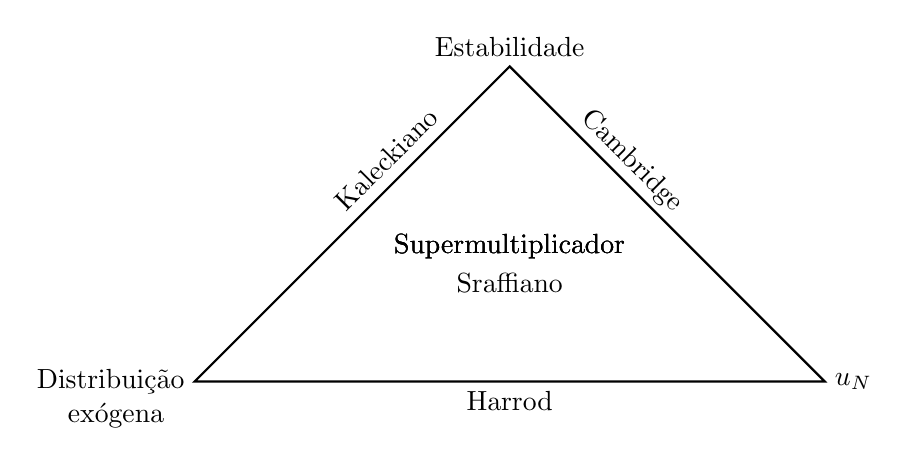
\begin{tikzpicture}[thick]
			\path[draw] (-4,0)  coordinate [label= left:Distribuição] (A)
			
			-- ( 0,4)  coordinate [label=above:Estabilidade] (C)
			-- ( 4,0)  coordinate [label=right:$u_N$] (B)
			-- cycle;
			\foreach \point in {A,B,C}
			\draw
			-- (0,2) node[anchor=north]{Supermultiplicador};
			\draw
			-- (-5,-0.15) node[anchor=north]{exógena};
			\draw
			-- (0,1.5) node[anchor=north]{Sraffiano};
			\draw
			-- (-1.75,3) node[anchor=north, rotate=45]{Kaleckiano};
			\draw
			-- (1.75,3) node[anchor=north, rotate=-45]{Cambridge};
			\draw
			-- (0,0) node[anchor=north]{Harrod};
			\end{tikzpicture}
		}
	\end{center}
	\caption*{\textbf{Fonte:} Elaboração própria}
\end{figure}
\noindent Essa trindade impossível se mostrou falsa com o desenvolvimento do supermultiplicador sraffiano, proposto por \textcite{serrano_long_1995} e \textcite{bortis_institutions_1996}. Portanto, diante da discussão anterior, conclui-se que o modelo do SSM não é incompatível para analisar o médio prazo ou restrito ao longo prazo como afirma \textcite{nikiforos_comments_2018}. Com isso, encerra-se este capítulo elegendo o supermultiplicador sraffiano como o mais adequado por replicar os fatos estilizados mencionados anteriormente e por validar o PDE no curto, médio e longo prazo. Seguindo a sugestão de \textcite[p.~280]{freitas_growth_2015}, esta investigação avança no sentido de contribuir para a compreensção de outros componentes da demanda agregada não criadores de capacidade. Destaca-se ainda que a instabilidade da economia não decorre da junção do acelerador com o multiplicador\footnote{Como mostram \textcite{serrano_trouble_2017}, dadas certas condições, o SSM é dinamicamente \textit{estável}.}, mas sim da própria instabilidade da demanda agregada \cite{dejuan_hidden_2017}.
